\chapter{Results}\label{chapter:results}

In this chapter I introduce how my CUDA pressure solver cuts the simulation speed against the CPU and the $\Phi_{flow}$ implementation. I also compare the error caused by floating point errors on GPUs.
\par All tests were performed in a closed boundary environment with random divergence vectors in the $\left[-1, 1 \right]$ range. Before starting the measurement, a warm-up of 10 solutions was performed. The data show the average of 100 

\begin{figure*}[t]
    \centering
	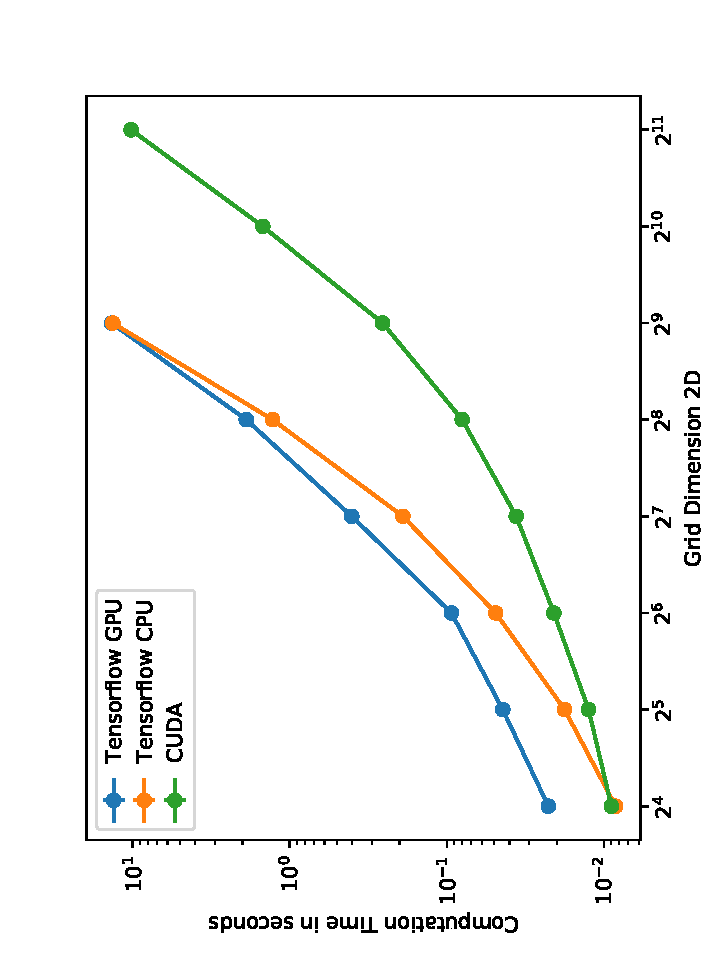
\includegraphics[scale=1.15]{figures/Benchmark2D}

	\caption{Pressure Solve in 2D}
\end{figure*}
\begin{figure*}[t]
    \centering
	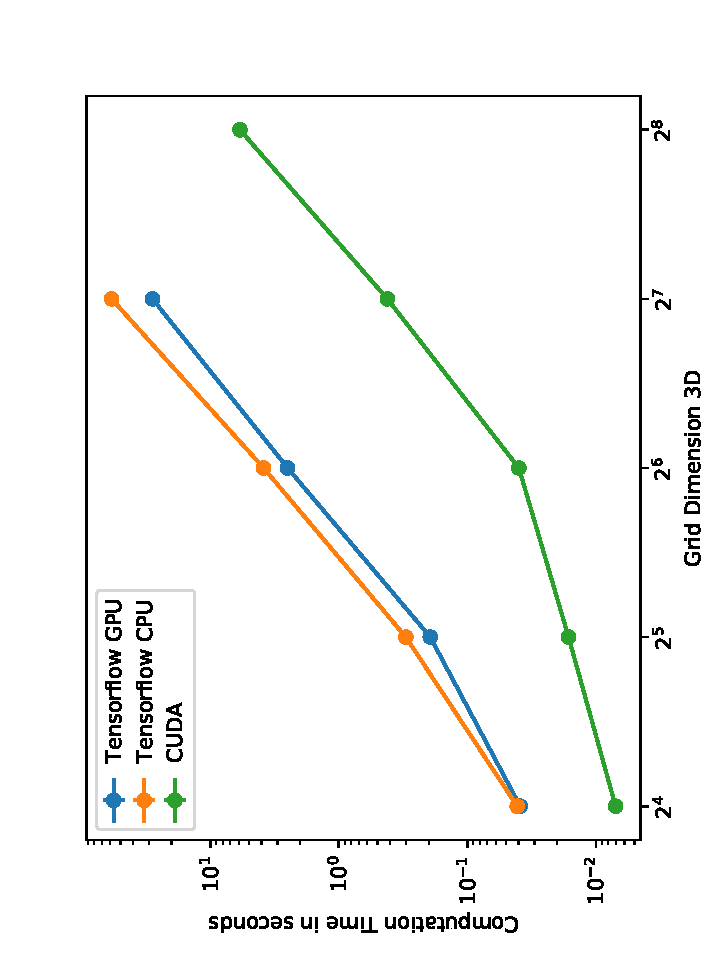
\includegraphics[scale=1.15]{figures/Benchmark3d}

	\caption{Pressure Solve in 3D}
\end{figure*}